\documentclass[12pt,a4paper]{article}

% ---------- Encoding & language ----------
\usepackage[utf8]{inputenc}
\usepackage[T1]{fontenc}
\usepackage[romanian]{babel}
\usepackage{lmodern}

% ---------- Page layout & typography ----------
\usepackage[a4paper, margin=2.5cm]{geometry}
\usepackage{microtype}
\usepackage{parskip}
\usepackage{setspace}

% ---------- Graphics, tables, math ----------
\usepackage{graphicx}
\usepackage{amsmath}
\usepackage{array}
\usepackage{booktabs}
\usepackage{longtable}
\usepackage{tabularx}
\usepackage{multirow}
\usepackage{xcolor}
\usepackage{float}
\usepackage{pgfgantt}
\usepackage[official]{eurosym}

% ---------- Lists & enumeration ----------
\usepackage{enumitem}
\setlist{itemsep=2pt, topsep=4pt}

% ---------- Hyperlinks ----------
\usepackage{hyperref}
\hypersetup{
    colorlinks=true,
    linkcolor=black,
    urlcolor=blue!60!black,
    citecolor=black,
    pdftitle={PharmacoAI -- Business Foundation},
    pdfauthor={Echipa PharmacoAI}
}

% ---------- Document-wide commands ----------
\newcommand{\source}[1]{\textit{\small (#1)}}

\begin{document}

% ---------- Custom title page ----------
\begin{titlepage}
\thispagestyle{empty}
\centering

\vspace*{0.5cm}

{\small\scshape Universitatea din București \par Facultatea de Matematică și Informatică \par}
% {\small\itshape Managementul Proiectelor Agile (MPA), 2026 \par}

\vspace{1.2cm}

{\color{blue!60!black}\rule{\linewidth}{1.2pt}}

\vspace{0.6cm}

{\Huge\bfseries PharmacoAI \par}
\vspace{0.4cm}
{\Large Plan de afaceri \par}
{\large\itshape Asistent agentic pentru farmacii \par}

\vspace{0.4cm}

{\color{blue!60!black}\rule{\linewidth}{0.8pt}}

\vspace{1.2cm}


\includegraphics[width=0.42\textwidth]{Gemini_Generated_Image_ic7cxaic7cxaic7c.png}

\vspace{0.8cm}

{\large\itshape ,,Intelligence that heals. Innovation that scales.''\par}

\vfill

{\large\bfseries Autori \par}
\vspace{0.3cm}
\begin{tabular}{c}
    Cucu Raul-Mihai \\[0.2em]
    Ghinea Dragoș-Dumitru \\[0.2em]
    Ghergu Ioana-Laura \\
\end{tabular}

\vspace{1cm}

{\small \today \par}

\end{titlepage}
\tableofcontents
\newpage

% ---------- Capitole ----------
\section{Rezumat executiv}

\subsection*{Motto}
\textit{,,Intelligence that heals. Innovation that scales.''}

\subsection*{Propunerea de valoare}
PharmacoAI este un asistent software \textbf{agentic} pentru farmacii, integrat în activitatea zilnică la ghișeu, care îl ajută pe farmacist să răspundă rapid și corect la întrebări legate de medicamente, interacțiuni și mod de utilizare. Aplicația transformă o întrebare liberă a clientului într-un răspuns verificat, sintetizat și adaptat la nivelul interlocutorului, într-un singur flux operațional.

\subsection*{Motivația aplicației}
Nevoia fundamentală care stă la baza dezvoltării PharmacoAI derivă dintr-o problemă critică și constantă a sistemului de sănătate: presiunea imensă asupra timpului farmaciștilor, combinată cu necesitatea vitală a pacienților de a avea acces rapid la informații sigure și clare despre medicația lor. În prezent, farmaciștii gestionează volume mari de clienți, ceea ce poate limita timpul acordat consultanței detaliate.

PharmacoAI intervine exact în acest punct nevralgic, propunând o soluție care eficientizează interacțiunea farmacist-pacient. Prin utilizarea unei arhitecturi inovatoare de tip \textbf{Agentic Workflow} (agenți AI multipli, specializați pe sarcini clare), aplicația adresează direct cea mai mare vulnerabilitate a tehnologiei în domeniul medical: \textbf{riscul de halucinație} a datelor și răspunderea legală severă. Această rigoare tehnică îi permite să opereze în siguranță, fiind utilă atât ca instrument de asistență rapidă pentru specialiști, cât și ca platformă de informare pentru clienți (\textit{dual audience capability}).

Mai mult, motorul avansat de \textbf{normalizare a denumirilor de medicamente} rezolvă provocări practice majore: corectează erorile de scriere și identifică instantaneu alternative, inclusiv echivalente internaționale. Astfel, PharmacoAI depășește stadiul de simplu asistent, devenind un instrument capabil să crească siguranța și calitatea actului farmaceutic, oferind opțiuni flexibile și scalabile de integrare pentru farmaciile de orice dimensiune.

\subsection*{Indicatori-cheie ai planului}
\begin{itemize}
    \item \textbf{Investiție inițială (MVP, 6 luni):} $\sim$20.000~\euro
    \item \textbf{Capital total investit până la break-even:} $\sim$65.600~\euro
    \item \textbf{Perioadă de recuperare estimată:} $\sim$2 ani și 9 luni
    \item \textbf{Venit anual estimat în Anul 3:} $\sim$180.000~\euro
    \item \textbf{Marjă brută software:} peste 95\,\% (la pachetul Pro)
\end{itemize}

\section{Produsul și utilizatorii}

\subsection{Descrierea produsului}
PharmacoAI este construit pe un sistem de agenți specializați: un \textbf{agent general} primește mesajul clientului (scris sau citit automat), decide dacă întrebarea poate fi răspunsă imediat sau dacă necesită un ,,flux de analiză medicală'' și, în cazul complex, lansează o secvență de pași specializați:

\begin{itemize}
    \item \textbf{Agent de normalizare a medicației}: corectează denumirea greșită, identifică ingredientul activ și găsește analoge/similare în alte țări.
    \item \textbf{Agent de \textit{facts}}: consultă mai multe baze de date pentru informații despre indicații, contraindicații, efecte adverse și interacțiuni.
    \item \textbf{Agent de sinteză}: rezumă datele într-un răspuns clar, profesional, pentru farmacist.
    \item \textbf{Agent de traducere pentru pacient}: transformă răspunsul profesional într-un text pe înțelesul unui utilizator obișnuit, fără jargon medical.
\end{itemize}

În esență, PharmacoAI oferă un serviciu de asistență agențială pentru farmacii care transformă o întrebare liberă a clientului într-un răspuns verificat, sintetizat și adaptat la nivelul de cunoștințe al interlocutorului, într-un singur flux integrat în operațiunea zilnică a farmaciei.

\subsection{Utilizatori-țintă și \textit{user stories}}

\paragraph{Farmacist (utilizator principal).}
\begin{itemize}
    \item Vreau să pot citi rapid informații corecte despre un medicament nou sau rar, fără să navighez între mai multe resurse externe, astfel încât să răspund clientului în mai puțin de 30 de secunde.
    \item Vreau ca sistemul să îmi spună automat dacă două medicamente pot fi luate împreună și care sunt riscurile majore, pentru a evita prescripții periculoase.
    \item Vreau să pot introduce numele unui medicament scris greșit sau incomplet și să primesc automat denumirea corectă și ingredientul activ, astfel încât să nu risc confuzii la vânzare.
    \item Vreau să pot oferi pacientului un răspuns clar și simplu, generat de sistem, în loc să compun singur explicații în fiecare caz, pentru a economisi timp și a reduce riscul de erori.
\end{itemize}

\paragraph{Administrator de lanț de farmacii.}
\begin{itemize}
    \item Vreau să pot gestiona un cont central pentru mai mulți utilizatori, astfel încât să mențin sub control organizarea internă.
\end{itemize}

\paragraph{Pacient (utilizator final).}
\begin{itemize}
    \item Vreau să primesc răspunsuri clare, înțelese de oricine, la întrebări simple despre medicamente, dozaj sau interacțiuni, fără a fi nevoit să citesc texte tehnice sau complicate.
\end{itemize}

\section{Stiva tehnologică}

PharmacoAI este organizat ca un sistem pe trei niveluri: o aplicație single-page \textbf{React + Vite}, un backend \textbf{FastAPI (Python 3.13)} care expune endpoint-uri REST și de \textit{streaming} (Server-Sent Events), și un server dedicat \textbf{Model Context Protocol (MCP)} care intermediază accesul la unelte pentru agenții AI. Cele trei servicii sunt configurate prin variabile de mediu (\texttt{.env} comun) și sunt pornite local printr-un script PowerShell unificat.

\begin{table}[H]
\centering
\small
\renewcommand{\arraystretch}{1.15}
\begin{tabular}{p{3.2cm}p{11cm}}
\toprule
\textbf{Strat} & \textbf{Tehnologii și responsabilități} \\
\midrule
Frontend & React 18, Vite 5, \texttt{react-markdown} (cu GFM): landing page, chat farmacist cu \textit{streaming}, panou admin utilizatori, fluxuri cont și facturare. \\
Backend API & FastAPI 0.115, Uvicorn (ASGI), Pydantic v2, \texttt{httpx}: autentificare, RBAC (admin / farmacist), \textit{tier}-uri de abonament, persistență, logare structurată, livrare prin SSE cu suport pentru anulare. \\
Persistență & Repository pe fișiere JSON, interschimbabil cu o bază de date administrată fără modificări de interfață. \\
Strat AI / Agenți & Multipli agenți \textbf{Google Gemini} (\texttt{gemini-3-flash-preview}) într-un \textit{pipeline} de tip triere $\rightarrow$ normalizare $\rightarrow$ evidențe $\rightarrow$ sinteză, cu \textit{handoff} între agenți; configurare declarativă (prompt, model, temperatură, nivel de risc). \\
Server MCP & FastMCP (Python SDK MCP), transport HTTP \textit{streaming}; expune unelte de evidență medicamentoasă cu cache, \textit{audit log}, \textit{rate limiting} și detectare a contextului clinic incomplet. \\
Surse de date medicale & openFDA Drug Label, RxNorm (NLM), DailyMed (NLM). \\
Plăți & Stripe Checkout pentru abonamente și pachete de mesaje, cu validarea semnăturii \textit{webhook}-urilor. \\
Tooling & Python \texttt{venv} + \texttt{pip}, \texttt{npm}, Git, OpenAPI/Swagger auto-generat la \texttt{/docs}. \\
\bottomrule
\end{tabular}
\caption{Sumar al stivei tehnologice}
\label{tab:stack}
\end{table}

Arhitectura este \textbf{API-first} și \textbf{configuration-driven}: agenții și uneltele MCP pot fi adăugate sau înlocuite fără modificări la nivelul frontend-ului, iar restricțiile de acces (ce agenți și câte mesaje pot fi consumate) sunt centralizate în definițiile de \textit{tier}. Această separare permite rularea aplicației atât pe modele \textit{cloud} (Gemini) cât și, ulterior, pe modele \textit{open-source} găzduite pe GPU dedicat, cu efort minim de migrare.

\section{Analiza SWOT}

\subsection{Puncte tari (\textit{Strengths})}
\begin{itemize}
    \item \textbf{High-value use case}: industria farmaceutică gestionează o nevoie umană critică și recurentă. Întrebări despre medicamente sunt puse zilnic, iar existența unei soluții care să eficientizeze timpul de interacțiune al farmacistului cu clienții este esențială.
    \item \textbf{Agentic Workflow}: utilizarea mai multor agenți specializați în favoarea unui singur agent generic crește acuratețea răspunsurilor și scade riscul de halucinare.
    \item \textbf{Flexible monetization}: farmaciile independente sau mai puțin dezvoltate pot integra soluția prin planul \textit{Starter} accesibil (de la 10\,\$/lună) și prin pachete suplimentare de mesaje \textit{pay-as-you-go}, fără un angajament financiar mare la început.
    \item \textbf{Dual audience capability}: farmaciile pot pune serviciul la dispoziția clienților prin contul de farmacist; clienții se pot informa și individual despre medicamentele pe care le consumă.
    \item \textbf{Medication normalization engine \& cross-country drug alternatives}: sistemul identifică medicamente și ingrediente în pofida greșelilor de scriere, oferă alternative locale și echivalente disponibile în alte țări.
\end{itemize}

\subsection{Puncte slabe (\textit{Weaknesses})}
\begin{itemize}
    \item \textbf{Data dependency}: agentul de \textit{facts} are nevoie de baze de date cu medicamente și ingrediente care să conțină informații corecte și să fie actualizate periodic.
    \item \textbf{Bariera de adoptare}: farmaciștii sunt presați de timp și lucrează cu volume mari de clienți zilnic; pot fi reticenți în a integra un instrument suplimentar dacă acesta nu este integrat în sistemul de gestiune existent.
    \item \textbf{High liability risk}: halucinațiile legate de dozaje sau interacțiuni medicamentoase, însoțite de neatenție umană, pot pune în pericol viața consumatorilor și pot atrage consecințe legale.
\end{itemize}

\subsection{Oportunități (\textit{Opportunities})}
\begin{itemize}
    \item \textbf{Expansiune către industria cosmetică}: soluția poate fi extinsă pentru a explica ingredientele din produsele cosmetice și potențialele riscuri adverse.
    \item \textbf{Integrare ERP / Gestiune}: soluția poate fi integrată cu softurile de gestiune farmaceutică și poate oferi alternative de medicamente bazate pe stocurile existente.
    \item \textbf{Internaționalizare}: motorul de echivalențe trans-frontaliere deschide piețe în care turismul medical sau migrația cresc cererea pentru identificarea de alternative locale.
\end{itemize}

\subsection{Amenințări (\textit{Threats})}
\begin{itemize}
    \item \textbf{Reglementări stricte din domeniul medical}: pot restricționa sau elimina utilizarea AI în consultanță medicală (ex.: AI Act în UE).
    \item \textbf{Negative perception of AI in medical contexts}: atât farmaciștii, cât și clienții, pot fi sceptici în a adopta o soluție bazată pe AI când vine vorba de sănătate, preferând să se bazeze pe specialiști.
    \item \textbf{Concurența Big Pharma}: companiile mari ar putea intra pe piață cu propriile soluții și ar putea fi preferate datorită renumelui deja stabilit.
\end{itemize}

\section{Analiza de piață}

\subsection{Principalii competitori}

\paragraph{Sully.ai.} Se poziționează ca ,,AI Pharmacist'' pentru organizații medicale, cu accent pe verificarea medicației, verificarea interacțiunilor, managementul prescripțiilor și integrarea cu sisteme EHR (Epic, AthenaHealth, Cerner). Este puternic pe automatizare clinică și integrare \textit{enterprise}, dar orientat mai ales către spitale și sisteme mari, nu către farmacii comunitare.

\paragraph{Pharmie AI.} Axat pe farmacii independente și pe automatizarea apelurilor, cererilor de \textit{refill}, întrebărilor despre asigurări, stoc și campanii \textit{outbound}. Soluție valoroasă operațional, dar accentul cade pe comunicații și \textit{front-desk}, nu pe analiză medicamentoasă multi-agent și sinteză clinică.

\paragraph{Asepha.ai.} Construit în jurul automatizării procesării prescripțiilor și documentelor, folosind OCR pentru rețete scrise de mână, extragerea datelor și verificări de interacțiuni. Este puternic pe \textit{back-office} și eficiență administrativă, dar nu este orientat în primul rând spre conversația farmacist-pacient.

\paragraph{Pharmesol.} ,,AI Pharmacy Agent'' pentru echipele din farmacii, cu accent pe automatizarea apelurilor, mesajelor, documentării și fluxurilor operaționale. Se integrează cu Pharmacy Management System, telefonie și \textit{scheduling}.

\paragraph{PharmacyAI.} Aplicație orientată mai degrabă către utilizatorul final decât către farmacie. Funcționalități: verificarea interacțiunilor, căutare de informații, asistent AI multilingv, remindere, listă personală de medicamente și scanare foto. Este construit ca asistent mobil personal.

\subsection{Matricea de funcționalități}

\begin{table}[h!]
\centering
\small
\setlength{\tabcolsep}{4pt}
\renewcommand{\arraystretch}{1.2}
\resizebox{\textwidth}{!}{%
\begin{tabular}{|p{4.2cm}|c|c|c|c|c|c|}
\hline
\textbf{Funcționalitate} & \textbf{PharmacoAI} & \textbf{Sully.ai} & \textbf{Pharmie AI} & \textbf{Asepha.ai} & \textbf{Pharmesol} & \textbf{PharmacyAI} \\
\hline
Asistent conversațional general & DA & Parțial & DA & Parțial & DA & DA \\
\hline
Corectare/normalizare nume medicament & DA & NU & NU & Parțial & NU & Parțial \\
\hline
Identificare ingrediente active & DA & Parțial & Limitat & Parțial & NU & Parțial \\
\hline
Alternative similare în alte țări & DA & NU & NU & NU & NU & NU \\
\hline
Căutare informații în multiple baze de date & DA & Parțial & NU & NU & NU & NU \\
\hline
Sinteză automată a răspunsului medical & DA & Parțial & Limitat & Limitat & Parțial & DA \\
\hline
Traducere în limbaj uzual pentru pacient & DA & Limitat & Parțial & Limitat & DA & DA \\
\hline
Verificare combinații / interacțiuni & DA & DA & Limitat & DA & NU & DA \\
\hline
Informații despre dozaj & DA & Parțial & Limitat & Parțial & NU & NU \\
\hline
Subscripții multi-user & DA & NU & NU & NU & NU & NU \\
\hline
Top-up de mesaje & DA & NU & NU & NU & NU & NU \\
\hline
Acces pentru \textit{end-customer} & DA & NU & DA & Parțial & DA & DA \\
\hline
\end{tabular}%
}
\caption{Matricea comparativă a funcționalităților PharmacoAI vs. competiție}
\label{tab:matrice_competitori}
\end{table}

\subsection{Avantaje competitive}
\begin{itemize}
    \item Reunește într-un singur flux funcții care în piață sunt dispersate între baze de date, verificatoare de interacțiuni și \textit{chatboți} operaționali.
    \item Soluția este proiectată pentru farmacie ca \textbf{echipă}, nu doar pentru un clinician individual.
    \item Poate funcționa atât \textbf{B2B} (către farmacii), cât și \textbf{B2B2C} (dacă farmacia alege să lase clienții să interacționeze prin contul propriu).
    \item Găsirea alternativelor pentru un medicament specific este o soluție unică pe piață.
\end{itemize}

\subsection{Dezavantaje competitive}
\begin{itemize}
    \item Valoarea produsului depinde critic de calitatea bazelor de date medicale și de actualizarea lor continuă, iar competitorii consacrați au deja brand și credibilitate de conținut.
    \item Funcții precum recomandări de dozaj sau verificarea combinării medicamentelor intră într-o zonă sensibilă de conformitate, responsabilitate profesională și reglementare, ceea ce impune mecanisme de \textit{disclaimer}, \textit{audit trail} și supraveghere umană.
    \item Pentru competitorii \textit{enterprise}, avantajul integrării native în EHR/PMS poate fi greu de egalat în fazele incipiente ale startup-ului.
    \item Nivel redus de încredere în uneltele farmaceutice bazate pe AI.
\end{itemize}

\subsection{Diferențiator-cheie}
\begin{quote}
\textbf{PharmacoAI este singura soluție de pe piață care oferă alternative locale și echivalente internaționale pentru un medicament dat, integrate într-un flux conversațional adresat simultan farmacistului și pacientului.}
\end{quote}

\section{Analiza riscurilor}

Această secțiune rezumă riscurile critice ale proiectului, tipologia, impactul, probabilitatea de apariție și planurile de răspuns.

\subsection{Dozaj incorect și halucinații ale AI (\textit{Liability Risk})}
\begin{itemize}
    \item \textbf{Identificare:} Din cauza erorilor inerente în sistemele AI sau a datelor de antrenament imperfecte, aplicația poate oferi dozaje greșite, interacțiuni medicamentoase eronate sau informații false (halucinații). Acest risc este strâns legat de dependența de date.
    \item \textbf{Tip:} Tehnic (funcționare AI) și Business (reputație, legal).
    \item \textbf{Impact:} \textbf{Critic}. poate periclita viața pacienților, atrage acțiuni în instanță, pierderea încrederii în brand și, posibil, închiderea afacerii.
    \item \textbf{Probabilitate:} Medie.
    \item \textbf{Plan de răspuns:}
    \begin{itemize}
        \item \textit{Mitigare (prevenire):} arhitectură \textit{Agentic AI} cu straturi de validare încrucișată; audituri periodice ale bazelor de date; model \textit{human-in-the-loop} pentru informațiile critice; \textit{disclaimer}-e clare privind caracterul consultativ al răspunsurilor.
        \item \textit{Contingență (reacție):} asigurare de răspundere civilă profesională robustă și plan de comunicare de criză.
    \end{itemize}
\end{itemize}

\subsection{Adoptare scăzută în rândul farmaciștilor (\textit{Adoption Barrier})}
\begin{itemize}
    \item \textbf{Identificare:} Farmaciștii, deja supraîncărcați, pot fi reticenți în a integra un instrument suplimentar dacă nu este integrat nativ în sistemul lor de gestiune.
    \item \textbf{Tip:} Business (piață / vânzări) și Proiect (implementare).
    \item \textbf{Impact:} \textbf{Ridicat}. produsul nu va genera venituri, efortul de dezvoltare va fi irosit, iar proiectul ar putea eșua.
    \item \textbf{Probabilitate:} Ridicată.
    \item \textbf{Plan de răspuns:}
    \begin{itemize}
        \item \textit{Mitigare:} interfață extrem de intuitivă și rapidă; integrare prioritară cu software-urile ERP de gestiune farmaceutică; materiale educaționale și sesiuni de \textit{training} scurte; model de \textit{pricing} flexibil (plan \textit{Starter} accesibil și pachete \textit{pay-as-you-go}).
        \item \textit{Transfer:} parteneriate strategice cu asociații de farmaciști.
    \end{itemize}
\end{itemize}

\subsection{Reglementări stricte și schimbătoare}
\begin{itemize}
    \item \textbf{Identificare:} Autoritățile pot introduce legi care să limiteze sau să interzică utilizarea AI în consultanță medicală sau să impună cerințe costisitoare de certificare.
    \item \textbf{Tip:} Business (legal / conformitate).
    \item \textbf{Impact:} \textbf{Critic}. poate forța modificări fundamentale ale produsului sau interzicerea funcționării în anumite jurisdicții.
    \item \textbf{Probabilitate:} Medie spre Ridicată.
    \item \textbf{Plan de răspuns:}
    \begin{itemize}
        \item \textit{Mitigare:} colaborare cu experți legali specializați; urmărirea activă a legislației (ex.: AI Act UE); principii de \textit{compliance-by-design}; pivotare către industria cosmetică ca alternativă.
    \end{itemize}
\end{itemize}

\subsection{Dependența de date și întârzieri în actualizări}
\begin{itemize}
    \item \textbf{Identificare:} Agentul de \textit{facts} depinde de baze de date externe; întârzierile sau informațiile incomplete pot duce la erori.
    \item \textbf{Tip:} Tehnic (sistem) și Proiect (operare).
    \item \textbf{Impact:} \textbf{Mediu spre Ridicat}. informațiile depășite reduc valoarea produsului și cresc riscul legal.
    \item \textbf{Probabilitate:} Medie.
    \item \textbf{Plan de răspuns:}
    \begin{itemize}
        \item \textit{Mitigare:} acorduri SLA stricte cu furnizorii de baze de date; procese automate de verificare și integrare a actualizărilor; afișarea transparentă a datei ultimei actualizări.
    \end{itemize}
\end{itemize}

\subsection{Concurența companiilor Big Pharma}
\begin{itemize}
    \item \textbf{Identificare:} Companii farmaceutice mari, cu resurse vaste și branduri consacrate, ar putea dezvolta propriile soluții AI.
    \item \textbf{Tip:} Business (competitivitate).
    \item \textbf{Impact:} \textbf{Ridicat}. ar putea oferi produse superioare sau gratuite, bazându-se pe încrederea deja stabilită.
    \item \textbf{Probabilitate:} Medie.
    \item \textbf{Plan de răspuns:}
    \begin{itemize}
        \item \textit{Mitigare:} agilitate și inovație rapidă pentru păstrarea avantajului tehnologic; concentrare pe nișa farmaciilor independente; explorarea de parteneriate cu Big Pharma (licențiere în loc de competiție).
    \end{itemize}
\end{itemize}

\section{Planificare}

\subsection{Echipa}

Echipa ipotetică a startup-ului este formată din \textbf{3 fondatori-tehnici}, fiecare cu un domeniu de responsabilitate distinct, plus o linie comună de \textit{R\&D} pentru direcțiile viitoare:

\begin{itemize}
    \item \textbf{Cucu Raul-Mihai} --- \textit{Frontend \& Account Management}: landing page, structuri de conturi și roluri, securitate, acces preferențial la agenți.
    \item \textbf{Ghinea Dragoș-Dumitru} --- \textit{Agenți AI \& MCP}: \textit{tooling} MCP, agenții specializați (general, normalizare, \textit{facts}, sinteză, traducere pentru pacient) și orchestrarea fluxului \textit{agentic}.
    \item \textbf{Ghergu Ioana-Laura} --- \textit{Billing \& Tiers}: sistem de taxare B2B, planuri \textit{Basic / Pro / Max / Enterprise}, mesaje extra (\textit{pay-as-you-go}), integrare Stripe, \textit{upgrade}-uri și administrare la nivel de organizație.
\end{itemize}

\subsection{Diagrama Gantt}

Calendarul livrabilelor pentru perioada \textbf{20 aprilie -- 15 mai 2026} este sintetizat în diagrama de mai jos. Direcțiile de \textit{R\&D} sunt planificate ca fază paralelă, după livrarea funcționalităților principale.

\begin{figure}[H]
\centering
\resizebox{\textwidth}{!}{%
\begin{ganttchart}[
    hgrid,
    vgrid,
    time slot format=isodate,
    x unit=0.6cm,
    y unit chart=0.8cm,
    title height=1,
    bar height=0.5,
    bar/.append style={fill=blue!40},
    group/.append style={fill=blue!70},
    milestone/.append style={fill=red}
]{2026-04-20}{2026-05-15}

\gantttitlecalendar{day} \\

% Raul
\ganttgroup{Cucu Raul - Mihai}{2026-04-20}{2026-05-15} \\
\ganttbar{Landing page research}{2026-04-20}{2026-04-21} \\
\ganttbar{Landing page implementare}{2026-04-22}{2026-04-24} \\
\ganttbar{Structura conturi si roluri utilizatori}{2026-04-25}{2026-04-27} \\
\ganttbar{Setari securitate cont + limite consum}{2026-04-28}{2026-05-01} \\
\ganttbar{Access preferential la agenti}{2026-05-02}{2026-05-05} \\

% Dragos
\ganttgroup{Ghinea Dragoș - Dumitru}{2026-04-20}{2026-05-15} \\
\ganttbar{MCP Tooling}{2026-04-20}{2026-04-21} \\
\ganttbar{General Assistant Agent}{2026-04-22}{2026-04-23} \\
\ganttbar{Normalization Medication Agent}{2026-04-24}{2026-04-25} \\
\ganttbar{Medication Facts Agent}{2026-04-25}{2026-04-26} \\
\ganttbar{Medication Synthesis Agent}{2026-04-27}{2026-04-28} \\
\ganttbar{Layman Translation Agent}{2026-04-29}{2026-04-30} \\
\ganttbar{Agent orchestration}{2026-05-01}{2026-05-05} \\

% Ioana
\ganttgroup{Ghergu Ioana - Laura}{2026-04-20}{2026-05-15} \\
\ganttbar{Sistem taxare B2B}{2026-04-20}{2026-04-22} \\
\ganttbar{Planuri Basic / Pro / Max / Enterprise}{2026-04-23}{2026-04-25} \\
\ganttbar{Mesaje extra / Pay as you go}{2026-04-26}{2026-04-28} \\
\ganttbar{Integrare Stripe}{2026-04-29}{2026-04-30} \\
\ganttbar{Upgrade conturi + admin organization}{2026-05-01}{2026-05-05} \\

% Future work
\ganttgroup{Direcții viitoare}{2026-04-20}{2026-05-15} \\
\ganttbar{A/B testing frontend + feedback utilizatori}{2026-05-08}{2026-05-15} \\
\ganttbar{Extensive R\&D agent flows si modele AI}{2026-05-08}{2026-05-15}

\end{ganttchart}%
}
\caption{Diagrama Gantt --- planificarea livrabilelor pe membri și direcții}
\label{fig:gantt}
\end{figure}

\section{Analiza costurilor și modelul de business}

\subsection{Analiza costurilor API (Generative AI)}

Folosind un \textit{Agentic Workflow}, fiecare mesaj utilizator implică, în medie, \textbf{5 request-uri} către model (router, căutare, raționament clinic, sinteză, verificare), cu o medie de 1.000 tokeni \textit{input} și 200 tokeni \textit{output} per request.

\begin{table}[H]
\centering
\small
\begin{tabular}{lcccc}
\toprule
\textbf{Model AI} & \textbf{\$ / 1M tok.} & \textbf{\$ / req.} & \textbf{\$ / mesaj} & \textbf{3.000 mesaje} \\
\midrule
Gemini 3.1 Pro     & 1{,}25 / 5{,}00   & 0{,}00225  & 0{,}01125 & 33{,}75 \\
Gemini 3.1 Flash   & 0{,}15 / 0{,}60   & 0{,}00027  & 0{,}00135 &  4{,}05 \\
Gemini 3.0 Flash   & 0{,}075 / 0{,}30  & 0{,}000135 & 0{,}00067 &  2{,}01 \\
Gemini Flash Lite  & 0{,}037 / 0{,}15  & 0{,}000067 & 0{,}00033 &  1{,}00 \\
\bottomrule
\end{tabular}
\caption{Compararea costurilor modelelor Gemini (intrare/ieșire, USD)}
\label{tab:costuri_ai}
\end{table}

\textbf{Concluzii:} Gemini 3.1 Pro este prea scump pentru toți agenții, dar poate fi păstrat pentru raționamentul clinic final. Gemini 3.1 / 3.0 Flash sunt \textit{sweet spot}-ul pentru \textit{router} și agenții de căutare. La \$2--\$4 cost API pentru un abonament de \$99 marja brută software depășește 95\,\%. Pe termen mediu, costurile pot fi reduse prin modele \textit{open-source} rulate local pe un server GPU dedicat ($\sim$150--250~\$/lună, zeci de mii de inferențe fără cost per request). Pentru început, recomandăm \textbf{Gemini 3.1 Flash}.

\subsection{Costuri estimate}

\begin{table}[H]
\centering
\small
\begin{tabular}{lr}
\toprule
\multicolumn{2}{l}{\textbf{Costuri inițiale (MVP, 6 luni)}} \\
\midrule
Salarii fondatori (3 $\times$ 1.000~\euro\ $\times$ 6 luni) & 18.000~\euro \\
Costuri legale și înființare                                 &  1.500~\euro \\
\textit{Hosting} + API (testare)                             &    500~\euro \\
\midrule
\textbf{Total investiție inițială}                           & \textbf{$\sim$20.000~\euro} \\
\bottomrule
\end{tabular}
\hspace{0.5cm}
\begin{tabular}{lr}
\toprule
\multicolumn{2}{l}{\textbf{Costuri operaționale lunare (Anul 1)}} \\
\midrule
Salarii fondatori (3 $\times$ 1.500~\euro)  & 4.500~\euro \\
\textit{Cloud hosting} (Vercel, DB)         &   100~\euro \\
API AI                                       &   100~\euro \\
Marketing B2B                                &   400~\euro \\
Contabilitate și diverse                     &   200~\euro \\
\midrule
\textbf{Total lunar / anual}                 & \textbf{5.300 / 63.600~\euro} \\
\bottomrule
\end{tabular}
\caption{Structura costurilor: investiție inițială și costuri operaționale}
\label{tab:costuri}
\end{table}

\subsection{Modelul de business și estimări de venit}

Modelul comercial este \textbf{SaaS B2B} (cu opțiune B2B2C prin contul de farmacist). Pachetele și proiecția de venituri pe 3 ani sunt centralizate în Tabelul~\ref{tab:venituri}.

\begin{table}[H]
\centering
\small
\begin{minipage}{0.42\textwidth}
\centering
\begin{tabular}{lcc}
\toprule
\textbf{Pachet}   & \textbf{\$/lună} & \textbf{Mesaje} \\
\midrule
Starter           & 10   & 150 \\
Pro               & 99   & 3.000 \\
Ultimate          & 299  & 20.000 \\
\bottomrule
\end{tabular}
\par\smallskip\textit{Pachete de abonament}
\end{minipage}\hfill
\begin{minipage}{0.55\textwidth}
\centering
\begin{tabular}{lcccr}
\toprule
\textbf{An} & \textbf{Starter} & \textbf{Pro} & \textbf{Ultimate} & \textbf{Venit anual} \\
\midrule
1 & 20  & 15  &  0 & $\sim$18.000~\euro \\
2 & 40  & 50  &  2 & $\sim$72.000~\euro \\
3 & 80  & 120 & 10 & $\sim$180.000~\euro \\
\bottomrule
\end{tabular}
\par\smallskip\textit{Proiecție clienți și venituri}
\end{minipage}
\caption{Modelul comercial și estimarea veniturilor pe 3 ani}
\label{tab:venituri}
\end{table}

\subsection{Analiză cost / beneficiu}

\begin{table}[H]
\centering
\small
\begin{tabular}{lr}
\toprule
\textbf{Indicator} & \textbf{Valoare} \\
\midrule
Investiție MVP                          & 20.000~\euro \\
Pierdere Anul 1                         & $-$45.600~\euro \\
\textbf{Capital total investit}         & \textbf{65.600~\euro} \\
\midrule
Rezultat Anul 1 / 2 / 3                 & $-$45.600 / $+$2.000 / $+$80.000~\euro \\
\textit{Payback} (după pragul de profit) & $63.600 / 80.000 \approx 0{,}79$ ani \\
\textbf{Perioadă totală de recuperare}  & \textbf{$\sim$2 ani și 9 luni} \\
ROI la finalul Anului 3                 & $16.400 / 65.600 \times 100 \approx 25\,\%$ \\
\bottomrule
\end{tabular}
\caption{Indicatori financiari sintetici}
\label{tab:roi}
\end{table}

\section{Lean Canvas (1-page summary)}

\begin{figure}[H]
\centering
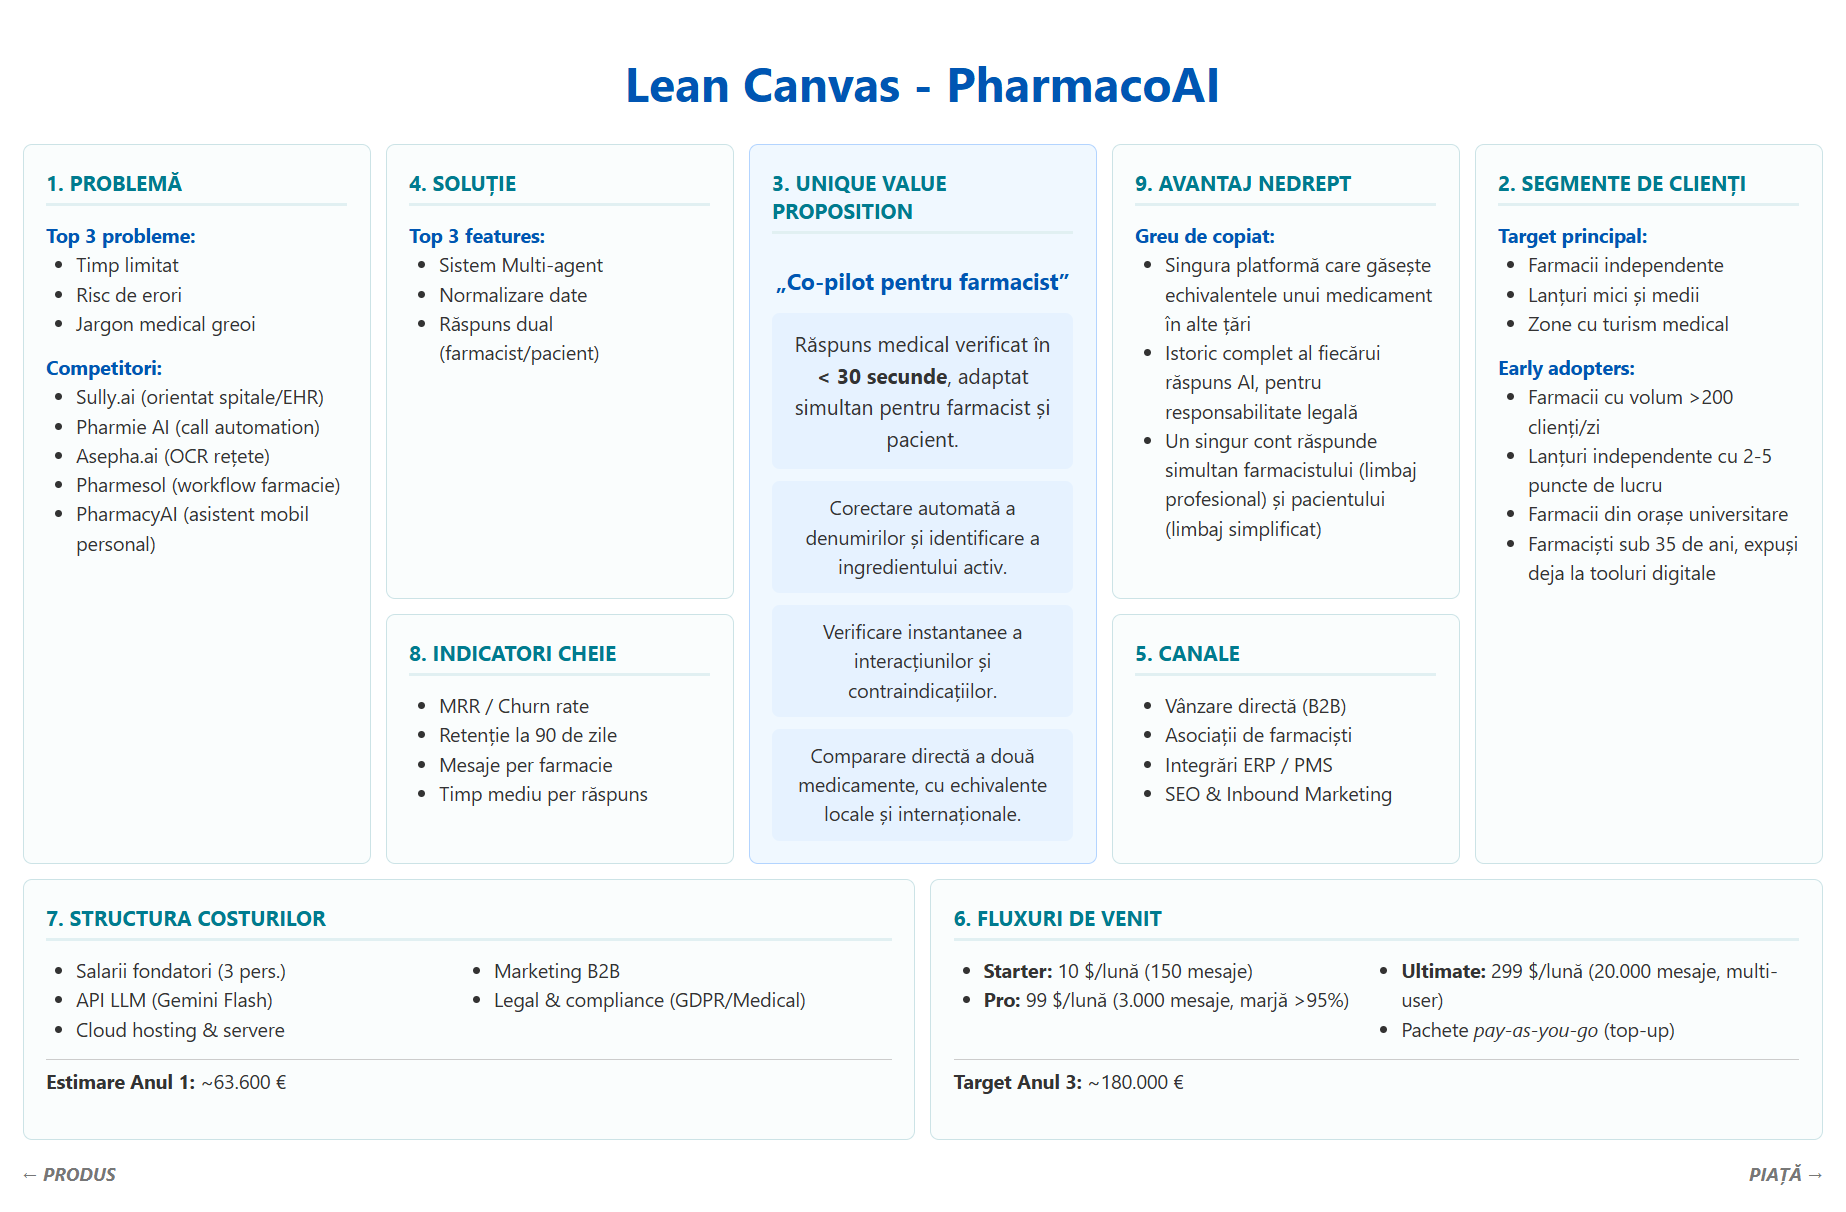
\includegraphics[width=\textwidth]{LeanCanvas.png}
\caption{Lean Canvas --- sinteză pe o pagină a modelului PharmacoAI}
\label{fig:lean_canvas}
\end{figure}

\section{Concluzii}

PharmacoAI răspunde unei nevoi reale și recurente a sistemului de sănătate: presiunea de timp asupra farmaciștilor și nevoia pacienților de informații medicale clare, sigure și ușor de înțeles. Soluția propusă combină o arhitectură tehnică modernă (\textbf{Agentic Workflow} peste un strat MCP integrat cu surse autoritative de date) cu un model comercial flexibil (SaaS B2B cu extensie B2B2C, plan \textit{Starter} de la 10\,\$/lună, pachete \textit{pay-as-you-go} și abonamente \textit{Pro} / \textit{Ultimate}).

Analiza competițională arată că, deși piața conține deja jucători importanți (Sully.ai, Pharmie AI, Asepha.ai, Pharmesol, PharmacyAI), niciunul nu acoperă \textbf{simultan}: normalizarea denumirilor, identificarea ingredientelor active, găsirea de alternative locale și internaționale, sinteza clinică și traducerea pentru pacient într-un singur flux conversațional. Acest \textbf{diferențiator-cheie}, cuplat cu suportul nativ pentru subscripții multi-utilizator și \textit{top-up} de mesaje, creează un teritoriu defensabil în special în nișa farmaciilor independente și a lanțurilor mici și mijlocii.

Din perspectivă financiară, modelul este \textbf{sustenabil}: o investiție inițială de $\sim$20.000~\euro\ pentru MVP, urmată de o pierdere normală în Anul 1, conduce la \textit{break-even} în jurul Anului 2 și la profitabilitate vizibilă din Anul 3 (ROI estimat $\sim$25\,\% la 3 ani, \textit{payback period} sub un an după depășirea pragului). Marja brută software ridicată ($>$95\,\%) și flexibilitatea de a migra parțial pe modele \textit{open-source} rulate local oferă un \textit{cushion} solid pentru scalare.

Riscurile principale (halucinații AI, bariera de adoptare, reglementări medicale și concurența \textit{Big Pharma}) sunt identificate explicit și au planuri de mitigare concrete (validare încrucișată, \textit{human-in-the-loop}, integrare ERP, \textit{compliance-by-design}, parteneriate strategice). Combinația dintre o propunere de valoare clară, o stivă tehnologică matură și un plan financiar realist face din PharmacoAI o investiție cu raport favorabil între risc și potențial de creștere.

\section*{Anexă: utilizarea uneltelor AI}
\addcontentsline{toc}{section}{Anexă: utilizarea uneltelor AI}

În realizarea acestui proiect am folosit pe scară largă unelte de tip \textit{generative AI} (modele Anthropic Claude, Google Gemini, OpenAI), atât pentru cod, cât și pentru documentație. În spiritul transparenței cerute de cursul MPA, declarăm explicit modul de utilizare:

\begin{itemize}
    \item \textbf{Aplicația este \textit{vibe-coded}.} Scheletul de cod (frontend React, backend FastAPI, integrare Stripe, persistență, fluxuri de autentificare) a fost generat și iterat prin sesiuni conversaționale cu asistenți AI, conform recomandării din cerințele cursului (,,vibe-codat cât mai mult posibil'').
    \item \textbf{Agenții sunt, de asemenea, \textit{vibe-coded}.} Definițiile agenților (\textit{system prompts}, parametrii de model, temperatura, niveluri de risc, \textit{tool wiring} către serverul MCP) și pipeline-ul de orchestrare (triere $\rightarrow$ normalizare $\rightarrow$ \textit{facts} $\rightarrow$ sinteză $\rightarrow$ traducere) au fost concepute și rafinate iterativ împreună cu modelele AI.
    \item \textbf{Documentația de față a fost revizuită cu AI.} Conținutul acestui document (rezumat executiv, SWOT, analiza de piață, riscuri, costuri, Lean Canvas, concluzii) a fost \textbf{scris de membrii echipei}, iar revizuirea, restructurarea, traducerea și formatarea LaTeX au fost realizate cu asistența unui model AI.
    \item \textbf{Codul a trecut prin multe iterații de intervenție umană.} Deși punctul de plecare al fiecărei componente a fost generat AI, forma finală reflectă numeroase iterații de revizuire, depanare, refactorizare și validare manuală efectuate de echipă; fără acest strat de intervenție umană, codul nu ar fi atins stadiul actual de funcționalitate, securitate și coerență arhitecturală.
\end{itemize}



\end{document}
